\documentclass{article}
\usepackage{../fasy-hw}

%% UPDATE these variables:
\renewcommand{\hwnum}{3}
\title{Discrete Structures, Homework \hwnum}
\author{Braeden Hunt (Tinnittin)}
\collab{n/a}
\date{due: 5 March 2021}

\begin{document}

\maketitle

This homework assignment should be
submitted as a single PDF file both to D2L and to Gradescope.

General homework expectations:
\begin{itemize}
    \item Homework should be typeset using LaTex.
    \item Answers should be in complete sentences and proofread.
    \item You will not plagiarize.
    \item List collaborators at the start of each question using the \texttt{collab} command.
    \item Put your answers where the \texttt{todo} command currently is (and
        remove the \texttt{todo}, but not the word \texttt{Answer}).
\end{itemize}


% ============================================
% ============================================
\collab{n/a} \nextprob{Good Proofs}
% ============================================
% ============================================

Look through proofs in this textbook, or other books / papers.  Define five
qualities that you think are common among good proofs. Provide citations to
examples.


\paragraph{Answer}

\todo{your answer here}



% ============================================
% ============================================
\collab{\todo{}} \nextprob{Max of a Subset}
% ============================================
% ============================================

Let $(B,\leq)$ be a totally ordered finite set. Prove the following
statement: For all subsets $A \subseteq B$, the following inequality
holds: $\max(A) \leq \max(B)$.

\paragraph{Answer}

\todo{your answer here}

% ============================================
% ============================================
\collab{\todo{}} \nextprob{Fibonacci}
% ============================================
% ============================================

The Fibonacci numbers are defined as follows:
$$
    F_i = \begin{cases}
            1 & i \in \{1,2\} \\
            F_{n-1}+F_{n-2} & \text{otherwise}
          \end{cases}
$$

Prove $\sum_{i=0}^n F_i = F_{n+2}-1$.

\paragraph{Answer}

\todo{your answer here}

% ============================================
% ============================================
\collab{\todo{}} \nextprob{US Coins}
% ============================================
% ============================================

Consider the four smallest denominations of US coins: $D=\{1,5,10,25\}$.  Prove, using
induction, that, for each $n \geq 1$, you can make $n$ cents using at most four
pennies.

\paragraph{Answer}

\todo{your answer here}

% ============================================
% ============================================
\collab{n\a} \nextprob{Four Colors Suffice}
% ============================================
% ============================================

Read Chapters $4$ and $5$ of \emph{Four Colors Suffice}.

Use a ``minimal criminal'' argument to prove that if an edge is removed from a
tree, then the resulting graph has two connected components.

        \paragraph{Answer}

	A tree is defined as a connected graph that has no cycles. It follows that there is one and only one path from one vertex to any other vertex.
	
	
	The base case is the simplest tree, a graph $G$ with two vertices connected by one edge. By removing the edge, the resulting graph has two connected components. See Figure \ref{graph}.
	
	
	Assume that a tree $P$ is structured is such a way that it satisfies the condition if an edge is removed from $P$, then the resulting graph has 
	two connected components and that if a tree $G$ is created by adding an edge to $P$, it does not satisfy that condition. This makes the graph $G$ a
	minimal criminal. We can see that this forms a contradiction, however, as by adding an edge to $P$ to create $G$, we are creating a cycle. We are 
	connecting two existing vertices with an edge, creating a direct path between them, but as $P$ is a tree, there is already a path between those two vertices.
	This means that there are two paths between the vertices. Therefore, $G$ is not a tree. Thus, the minimal criminal cannot exist.
	Because there is no minimal criminal and there is a base case, the statement is true.

 \begin{figure}
\caption{Base Case}
\centering
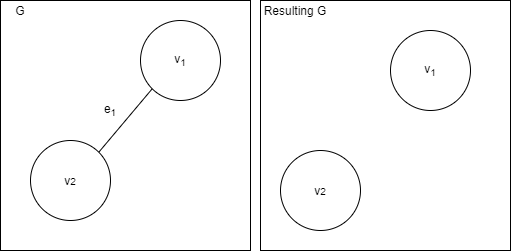
\includegraphics[width=0.5\textwidth]{images/graphBaseCase}
\label{graph}
\end{figure}

% ============================================
% ============================================
\collab{\todo{}}
\nextprob{Leonhard Euler}
% ============================================
% ============================================

Write a short (1-2 paragraph) biography of Leonhard Euler.
\textbf{In your own words}, describe who they are and why they are important in
the history of computer science.

If you use external resources, please provide
proper citations. If you do not use external sources, please write ``I did not
use any sources to write this biography'' as the last sentence of the
biography.

\paragraph{Answer}

\todo{your answer here}

% %% ... the bibliography
% \newpage
% \bibliographystyle{acm}
% \bibliography{biblio}

\end{document}

